% document style header
\documentclass[a4paper, 12pt]{config/homework}

% import default packages
\usepackage{config/defpackages}
% import custom math commands
\usepackage{config/domath}
\usepackage{pdfpages}

% end preamble
\begin{document}

% document title
\noindent
\begin{tabularx}{\textwidth}{>{\centering\arraybackslash}X>{\centering\arraybackslash}X>{\centering\arraybackslash}X}
Calvin Sprouse & PHYS489 3 & 2024 February 11\\
\midrule
\end{tabularx}

% homework problems begin
% Select and write a reflection on an artifact from your faculty-mentored undergraduate research experience. The artifact could include a project report, a print-out of a SOURCE presentation, or any other culminating product of your research project. In preparing your reflection, consider that research skills may include applying content knowledge to an original project; reading and referencing scientific literature; formulating a research goal; applying research methodology to address project goals; and disseminating your results.

% Scan your selected artifact(s) and combine these into a single PDF document.
% Prepare a 1/2 page reflection on how the artifact demonstrates your progress to meeting this goal
% Upload both pdf documents to Canvas by 11:59pm Friday, February 16.

Below is the culmination of my longest running research project working on computational simulations of pattern formation in axons. I started this research as an RUI in Summer 2022 and have made continual contributions ever since. I began this project having very little research experience and no biology experience. My computational experience made it possible for me to contribute immediately creating the animations shown in Figure 4 of the poster. Those animations developed my initial understanding of the system and as reading papers became less of a struggle and more of a stroll I've been able to approach more sophisticated questions. They have even been used to communicate ideas and results to experimental collaborators. This poster in particular is currently with me at the 2024 Biophysical Society Meeting where some of the qualitative behavior I first saw in the animations now has a quantitative description. With each presentation building up to the next I am excited for another opportunity to share this work. Already in the first day of the conference several presentations have inspired new ideas and investigations to this computational model. Upon returning from the conference this work will continue in an investigation of another incidental discovery from the animations which will take me through the summer. This project has leveraged and developed my skills in data analysis, simulation development, literature reviewing, presenting, data representation, and collaboration.

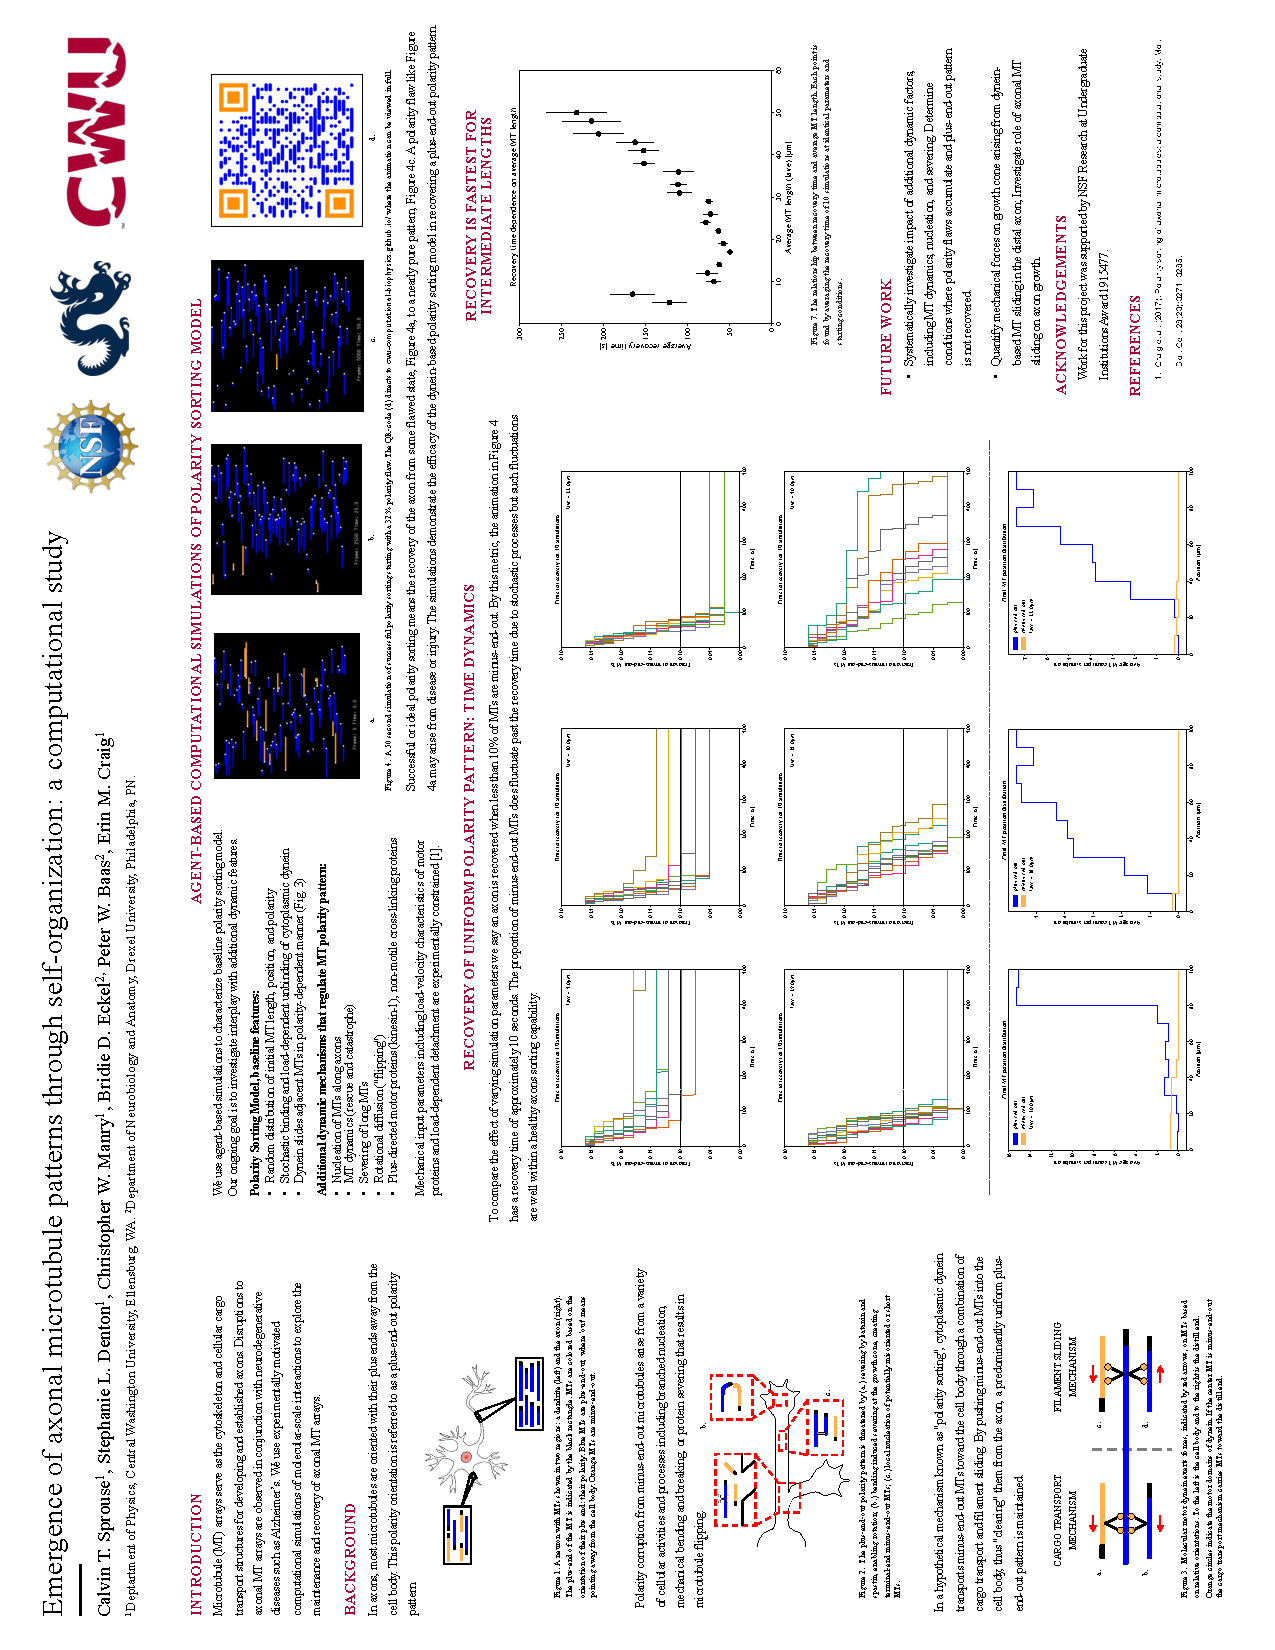
\includepdf[pages=-]{bps2024_cs_ds_poster_vFin.pdf}

\end{document}
